% !TeX spellcheck = it_IT
\documentclass[10pt,a4paper]{article}

\usepackage[utf8]{inputenc}
\usepackage[T1]{fontenc}	
\usepackage[italian]{babel}
\usepackage{amsmath}
\usepackage{amsfonts}
\usepackage{amssymb}
\usepackage{graphicx}

\usepackage[left=2cm,right=2cm,top=2cm,bottom=2cm]{geometry}
\geometry{a4paper}

\usepackage{booktabs} % for much better looking tables
\usepackage{verbatim}
\usepackage{subfig} % make it possible to include more than one captioned figure/table in a single 

\usepackage{fancyhdr} % This should be set AFTER setting up the page geometry
\pagestyle{fancy} % options: empty , plain , fancy
\renewcommand{\headrulewidth}{0pt} % customise the layout...
\lhead{}\chead{}\rhead{}
\lfoot{}\cfoot{\thepage}\rfoot{}

%%% SECTION TITLE APPEARANCE
\usepackage{sectsty}
%\allsectionsfont{\sffamily\mdseries\upshape} % (See the fntguide.pdf for font help)
% (This matches ConTeXt defaults)

% pacchetti che mi fanno schifo ma uso lo stesso (Bob è scemo, ma anche Ale...)
\usepackage[cdot, thickqspace, squaren]{SIunits}
% il miglior pacchetto che potessi desiderare
\usepackage{float}
% macro che mi piacciono
\def\code#1{\texttt{#1}}


\title{Esercitazione 8: Oscillatore sinusoidale a ponte di Wien con OpAmp}

\author{Gruppo BE \\ Alessandro Candido, Roberto Ribatti}
\date{\today}
\begin{document}
\maketitle

\section{Scopo e strumentazione}
Lo scopo dell'esperienza è realizzare un oscillatore ad onda sinusoidale a ponte di Wien utilizzando un OpAmp.

La strumentazione usata è quella presente sul banco di lavoro, più l'OpAmp TL081 e i diodi 1N1711.
%in realtà sia per l'OpAmp che per i diodi non abbiamo controllato che modello fossero, ce lo scriviamo comunque?

\section{Loop gain del circuito}
Si è disconnesso il circuito nel punto A, connettendo l'ingresso non-invertente dell'OpAmp al generatore di funzioni e osservando con l'oscilloscopio il segnale all'altro estremo rimasto disconnesso.
Si è in questo modo misurato il loop gain (modulo e fase) per varie frequenze immesse dal generatore di funzioni. Si riportano i grafici in \figurename{~\ref{fig:Bode}} e \figurename{~\ref{fig:fasi}}, e la tabella con i dati in appendice (\tablename{~\ref{tab:loop}}).

\begin{figure}[H]
	\begin{minipage}{\textwidth}
		\centering
		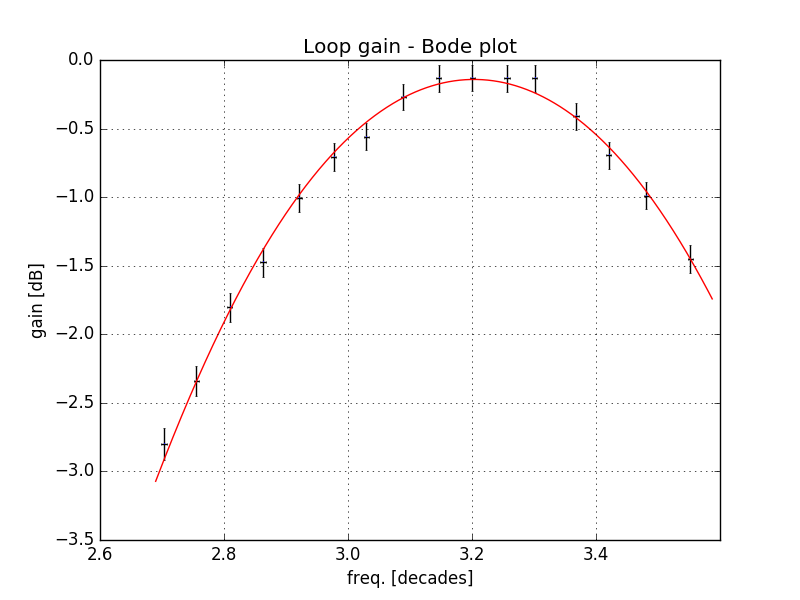
\includegraphics[width=0.8\textwidth]{../grafici/fit_loopgain_bode.pdf}
		\caption{Bode plot del guadagno di loop}
		\label{fig:Bode}
	\end{minipage}
\end{figure}

La frequenza a cui lo sfasamento si annulla è stata misurata e il valore è $f_0 = \unit{1.80 \pm 0.05}{\kilo\hertz}$.

Si è osservato che l'ampiezza del segnale di output dipende in modo monotono dalla posizione del potenziometro. In particolare la dipendenza osservata appariva lineare (affine). 

\section{Comportamento dell'output in funzione della posizione del potenziometro}
Si è riconnesso il circuito nel punto A e si è osservata la dipendenza del segnale in uscita in funzione della posizione del potenziometro.

\section{Frequenza di oscillazione}

\subsection{Dipendenza dalla posizione del potenziometro}
La frequenza di oscillazione è indipendente dalla posizione del potenziometro.

\subsection{Dipendenza dalla tensione di alimentazione}
La frequenza di oscillazione risulta indipendente dalla tensione di alimentazione, fintanto che questa non diventi abbastanza elevata da portare il segnale di output in clipping.

\section{Guadagno all'innesco dell'oscillazione}

\section{Scopo dei diodi}
Lo scopo dei diodi è di stabilizzare la tensione sull'output, in modo tale 
% chi è che lo mandava in saturazione, l'alimentazione o il potenziometro?

\pagebreak
\section{Appendice: Dati acquisiti}
Si riportano qui le tabelle dei dati usati per i fit e i grafici.
\centering
\begin{figure}[H]
	\centering
	\resizebox{0.7\textwidth}{!}{
	\input{../tabelle/tab_loopgain.txt}}
	\captionof{table}{Loopgain}
	\label{tab:loop}
\end{figure}




\end{document}
